%  LaTeX support: latex@mdpi.com
%=================================================================
% JRFM is an APA-style MDPI journal. The class loads mdpi_apacite and sets
% \bibliographystyle and \bibpunct itself, so neither is set here.
\documentclass[jrfm,article,submit,pdftex,moreauthors]{Definitions/mdpi}

%=================================================================
% MDPI internal commands - do not modify
\firstpage{1}
\pubvolume{1}
\issuenum{1}
\articlenumber{0}
\pubyear{2026}
\copyrightyear{2026}
\datereceived{ }
\daterevised{ }
\dateaccepted{ }
\datepublished{ }

\usepackage[table]{xcolor}
% ---------------------------------------------------------------------------
% DRAFTING MARKS.
%   \rev{...}  text added or rewritten in the current pass -- blue
%   \cut{...}  editorial note recording something removed  -- grey, bracketed
%   \todo{...} a section not yet drafted                   -- red, bracketed
% For a clean copy, redefine all three as \newcommand{\rev}[1]{#1},
% \newcommand{\cut}[1]{} and \newcommand{\todo}[1]{}.
% ---------------------------------------------------------------------------
\newcommand{\rev}[1]{{\color[HTML]{1A4E8C}#1}}
\newcommand{\CFix}[1]{{\color[HTML]{1A4E8C}#1}}
\newcommand{\cut}[1]{{\color[HTML]{6E6E6E}\small[removed in revision: #1]}}
\newcommand{\todo}[1]{{\color[HTML]{A31515}\small[to be drafted: #1]}}

% Figure search path: project root and figures/ subfolder
\graphicspath{{./}{figures/}}
%=================================================================

\Title{Beyond the Power Law: Log-Normal Bodies, Pareto Tails, and the Limits of
Industry Statistics}

\newcommand{\orcidauthorA}{0009-0004-4994-4800}
\newcommand{\orcidauthorB}{0009-0006-6831-426X}
\newcommand{\orcidauthorC}{0000-0002-3836-1851}

\Author{Sarthak Pattnaik $^{1}$\orcidA{}, Chhayank Jain $^{2}$\orcidB{}
and Eugene Pinsky $^{1,}$*\orcidC{}}

\address{%
$^{1}$ \quad Department of Computer Science, Metropolitan College,
Boston University, Boston, MA 02215, USA\\
$^{2}$ \quad Department of Computer Science, Arizona State University, Tempe, AZ 85281, USA}

\corres{Correspondence: epinsky@bu.edu}

\abstract{%
The claim that a power law governs the distribution of value in a digital economy is now
routine, and it is usually made at the level of the sector. We test it at three levels on
two censuses that between them cover every US employer firm from 1978 to 2023 and every
industry in the national accounts from 1997 to 2025, and the claim survives at only one of
them. Fitting a Pareto and a log-normal to interval-censored firm counts across ten size
classes by maximum likelihood, the log-normal is preferred by Vuong's test in all
forty-six years, at $|Z|$ above 200 throughout; the same fitted log-normal under-predicts
firms of 10{,}000 employees and over by a factor of twenty-one. The distribution is a
mixture, and the power law is a property of its tail alone: refitted from twenty employees
upward the exponent is 1.056, reproducing \citeauthor{Axtell2001}'s
(\citeyear{Axtell2001}) microdata estimate on binned data he did not use. At the sectoral
level the claim fails outright. Across 71 industries that tile the economy exactly once,
the association between how much value an industry creates and the share of it the industry
keeps is 0.009 by Pearson and $-0.047$ by Spearman: size buys no margin. A shift-share
decomposition of the forty-six-year rise in large-firm employment share attributes $+6.25$
percentage points to concentration rising inside sectors against $-6.38$ points from
employment moving toward less concentrated ones, so sectoral composition worked against the
trend rather than producing it. What did concentrate is capture rather than creation: the
Gini of operating surplus across industries exceeds that of value added in every year and
rose further, 0.587 to 0.627 against 0.512 to 0.551. Underneath all of this sits a measurement result we believe transportable. Every public
instrument censors its own upper tail. The largest firm-size class is open at 10{,}000
employees, the household income survey tops out at \$200{,}000, occupational wages stop
at the ninetieth percentile, and industry accounts average over the firms inside them.
Every concentration estimate reported here, and in the literature drawing on these
sources, is therefore a lower bound that cannot be tightened without microdata. A sector
average measures an object in which the phenomenon of interest has already been averaged
away.}

\keyword{firm size distribution; power law; Pareto tail; log-normal; interval-censored
maximum likelihood; business dynamism; industry concentration; value capture; Business
Dynamics Statistics; digital economy}

%%%%%%%%%%%%%%%%%%%%%%%%%%%%%%%%%%%%%%%%%%
\begin{document}

\maketitle

%%%%%%%%%%%%%%%%%%%%%%%%%%%%%%%%%%%%%%%%%%
\section{Introduction}
\label{sec:intro}

In 2023 the United States had 1{,}210 firms employing 10{,}000 people or more, out of 5.60
million employer firms in total. Fit a log-normal to the ten published size classes and it
expects 57. Fit a single Pareto and it expects 11{,}916. The first model wins the likelihood
comparison in every one of the forty-six years we examine, and it is wrong by a factor of
twenty-one about the firms that hold the economy's employment. The distribution of American firms is not one thing. Which of its two regimes an
estimate describes depends on where in the size range it was taken, and that is what
this paper is about.

\emph{Context and motivation.} The proposition that value in a digital economy follows a
power law has moved from the physics literature into general circulation, and it is now
usually asserted at the level of the sector: technology captures the returns, older
industries do not. The claim matters because it is doing work. It shapes how concentration
is described, which industries attract regulatory attention, and how the returns to
entrepreneurship are explained to the people considering it. It is also rarely tested at
the level at which it is asserted. The empirical literature on heavy tails works with
firms; the public argument works with sectors; and the two are not the same object.

\emph{What the literature establishes, and where it stops.} Four bodies of work bear on
this. The first, from \citet{Gibrat1931} and \citet{Simon1955} through \citet{Axtell2001}
and \citet{Luttmer2007}, establishes that the firm size distribution is heavy-tailed and
supplies growth-and-selection mechanisms that generate such tails. It has not settled what
the tail is: \citet{Axtell2001} finds an exponent indistinguishable from unity on the US
firm census, \citet{KondoLewisStella2023} reject the Zipf value on establishment microdata,
and \citet{ClausetShaliziNewman2009} show that samples of realistic size often cannot
discriminate between the candidate distributions at all. The second, running from
\citet{DunneRobertsSamuelson1988} to \citet{DeckerEtAl2016} and \citet{AkcigitAtes2021},
documents a long decline in firm entry and in the share of activity held by young firms.
The third, from \citet{Rosen1981} and \citet{FrankCook1995} to \citet{AutorEtAl2020} and
\citet{DeLoeckerEeckhoutUnger2020}, documents rising concentration and superstar dynamics,
usually with product-market shares or estimated markups. The fourth, in strategy rather
than economics, distinguishes creating value from capturing it \citep{Teece1986,
BrandenburgerStuart1996} and observes that the two need not travel together.

Each literature has a boundary the others do not cross. The distributional work is
overwhelmingly cross-sectional: a distribution is fitted at a point in time and an exponent
reported, so whether the shape moves is largely unexamined. The dynamism and concentration
work measures shares and rates rather than distributions, so it cannot say what functional
form is being deformed. The strategy literature is about firms and is not brought to
national data. And all of them draw on public statistics whose upper categories are open,
a limitation that is acknowledged case by case but has not, to our knowledge, been treated
as a systematic property of the evidence base.

\emph{The gap.} What is missing is a test of the same proposition at more than one level of
aggregation, on data covering the whole population rather than a listed subset, with an estimator
appropriate to how the data is published. The firm size distribution is
released as counts in size classes, which is interval-censored data; the industry accounts
are released as aggregates over firms. Neither supports the estimators the tail literature
usually reaches for, and treating a class midpoint as an observation or an industry mean as
a firm is how the levels get confused in the first place.

\emph{Research question and objectives.} The paper asks: \emph{is the distribution of value in the American economy governed by a power law, and
if so at what level: across the whole population of firms, in the upper tail of that
population, or between sectors?} Four
objectives follow. Fit competing distributions to interval-censored firm counts by maximum
likelihood and choose between them by a test appropriate to non-nested models. Establish
where in the size range a power law begins to hold, and how sensitive the resulting exponent
is to specification as against sampling. Decompose the change in concentration into a part
occurring within sectors and a part arising from employment moving between them. And measure
whether an industry's scale predicts the share of the value it creates that it retains.

\emph{Approach.} Two censuses are used. The Census Bureau's Business Dynamics Statistics
covers every US employer firm from 1978 to 2023 and reports counts and employment in ten
size classes and twelve age classes; the Bureau of Economic Analysis GDP-by-Industry
accounts report value added, gross output and the components of value added for the years
1997 onward. Both publish totals and subtotals mixed in with their components, and in both
cases the partition is recovered arithmetically and verified against the published total
before use. Distributions are fitted by multinomial maximum likelihood over intervals and
compared by \citeauthor{Vuong1989}'s (\citeyear{Vuong1989}) test; the tail is estimated by
the \citet{ClausetShaliziNewman2009} threshold procedure adapted to grouped data;
concentration is measured without distributional assumptions; and no estimator is used on
real data before recovering a planted answer from simulated data binned the same way.

\emph{Findings and contributions.} Three contributions follow, in the order the evidence
supports them.

First, the distributional claim fails and the tail claim holds, and the two are separable.
A log-normal is preferred over a Pareto in all forty-six years at $|Z|$ above 200, on counts
running to 5.60 million firms; the same log-normal under-predicts the largest class by a
factor of twenty-one. Refitted from twenty employees upward the Pareto exponent is 1.056,
within three thousandths of the microdata estimate of \citet{Axtell2001}, obtained here from
ten published bins by an estimator that never observes a firm. The distribution is a
mixture, and only its tail is a power law.

Second, the sectoral claim fails on two independent tests. Across 71 industries that tile
the economy exactly once, the association between how much value an industry creates and the
share of it the industry keeps is 0.009 by Pearson and $-0.047$ by Spearman. And a
shift-share decomposition of the forty-six-year rise in large-firm employment share
attributes $+6.25$ percentage points to concentration rising inside sectors against $-6.38$
points from employment moving toward less concentrated ones. Sectoral composition worked
against the trend rather than producing it. What did concentrate between sectors is capture
rather than creation: the Gini of operating surplus exceeds that of value added in every
year of the sample and rose further over the period.

Third, and this is a measurement result we believe transportable, every public instrument
bearing on the question censors its own upper tail, and it does so below the point at which
the tail becomes interesting. Because grouping can only reduce a concentration index, every
estimate reported here is a lower bound, and so is every comparable estimate in the
literature drawing on these sources. We also report a method that partially compensates: a
grouped tabulation that publishes its own total can be partitioned without labels, by
arithmetic, and the reconciliation is a test the analyst can fail rather than an assumption
they must make.

Section~\ref{sec:lit} places the exercise in the literature on firm size distributions,
business dynamism, concentration, value capture and the measurement of grouped data.
Section~\ref{sec:data} describes the two censuses and the partitions recovered from them.
Section~\ref{sec:method} sets out the estimators and what the design guards against.
Section~\ref{sec:results} reports the findings, and Section~\ref{sec:discussion} discusses
what they do and do not establish.

%%%%%%%%%%%%%%%%%%%%%%%%%%%%%%%%%%%%%%%%%%
\section{Literature Review}
\label{sec:lit}

\subsection{Heavy Tails in the Firm Size Distribution}
\label{subsec:lit_tails}

That firm sizes are distributed with a heavy upper tail is among the older regularities in
economics. \citet{Gibrat1931} proposed that growth rates are independent of size, which
generates a log-normal; \citet{Simon1955} showed that adding entry to a proportional-growth
process produces a Pareto tail instead. The two mechanisms differ in one assumption and
imply different distributions, and the empirical literature has spent seventy years trying
to tell them apart.

\citet{Axtell2001} gave the most cited answer, fitting the US firm census and obtaining a Pareto exponent statistically indistinguishable from unity, the value
\citet{Zipf1949} had described for word frequencies and \citet{Gabaix1999} later derived
for city sizes from a similar argument. \citet{Gabaix2009} surveys where such laws have
since been found across economics and finance. Theory followed:
\citet{Luttmer2007} shows that selection with entry and exit generates a tail near Zipf
under plausible parameters, and \citet{RossiHansbergWright2007} derive the size distribution
from the accumulation of industry-specific human capital. The tail also acquired
macroeconomic consequences. \citet{Gabaix2011} shows that when the firm size distribution is
sufficiently heavy-tailed, idiosyncratic shocks to individual firms do not wash out in
aggregate, an argument \citet{DiGiovanniLevchenko2012} extend to trade and country size using the
heterogeneous-firm framework of \citet{Melitz2003}.

The consensus is narrower than the citation count suggests.
\citet{CabralMata2003} document that the size distribution shifts systematically with firm
age, so a single cross-section confounds two things. \citet{Sutton1997} had already
catalogued how weakly the evidence constrains the underlying process.
\citet{KondoLewisStella2023}, working with establishment microdata, reject the Zipf value
outright and find a tail heavy but distinctly lighter than unity. And
\citet{ClausetShaliziNewman2009} showed that much of the disagreement is a measurement
artefact: the log-rank-on-log-size regression on which many estimates rest is biased, and
samples of the sizes commonly used often cannot separate a power law from a log-normal at
all. \citet{GabaixIbragimov2011} propose a correction to the regression estimator, and
\citet{Eeckhout2004} makes the parallel argument for cities, showing that a distribution
Zipf-like in its tail is log-normal over its full support.

Two things follow for the present paper. The question of whether a distribution is a power
law is separable from the question of whether its tail is, and the two require different
tests. And the estimator matters as much as the data: the results below use interval-censored
maximum likelihood precisely because the alternatives are either biased or unavailable on
data published as counts in classes.

\subsection{The Decline of Business Dynamism}
\label{subsec:lit_dynamism}

If entry is the mechanism by which firms reach the upper tail, then the rate of entry
governs how that tail is replenished. A large literature documents that the rate has fallen.

\citet{DunneRobertsSamuelson1988} established the basic patterns of entry and exit in US
manufacturing, and \citet{Hopenhayn1992} provided the equilibrium model in which entry, exit
and the size distribution are jointly determined. Using the same Longitudinal Business
Database that underlies the data in this paper, \citet{DeckerEtAl2014} document a
long-running decline in the startup rate, and \citet{DeckerEtAl2016} extend it across
sectors and regions. \citet{HaltiwangerJarminMiranda2013} establish why it matters: once firm age is
controlled for, the job-creating advantage commonly attributed to small firms belongs to
young ones, so a fall in entry is a fall in the economy's principal source of gross job
creation. \citet{FosterHaltiwangerKrizan2001} had already shown that reallocation
between entering, exiting and surviving plants accounts for a large share of aggregate
productivity growth, and \citet{DavisHaltiwanger2014} document that the flows themselves
have slowed across the labour market.

Explanations divide. \citet{DeckerEtAl2020} argue that the decline reflects reduced
responsiveness to shocks rather than smaller shocks, which points at rising adjustment
frictions. \citet{HopenhaynNeiraSinghania2022} show that slowing labour-force growth alone
can generate a lower entry rate, an older firm distribution and a rising concentration of
employment, so part of the pattern may be demographic rather than institutional.
\citet{PugsleySahin2019} trace the consequences for the business cycle, and
\citet{AkcigitAtes2021} assemble ten stylised facts and argue that a slowdown in the
diffusion of knowledge between leaders and followers accounts for most of them.
\citet{GuzmanStern2020} add an important qualification: the quantity of entrepreneurship
and its quality have moved differently, so a falling count of entrants is not by itself a
falling count of potential entrants to the tail.

What this literature measures is rates and shares. It establishes that entry has fallen and
that young firms hold less of the economy than they did, both of which we reproduce below.
It does not ask what has happened to the shape of the size distribution over the same
period, which is the question Section~\ref{subsec:tailresults} takes up.

\subsection{Concentration, Superstar Firms, and the Labour Share}
\label{subsec:lit_concentration}

A third literature documents rising concentration and connects it to the distribution of
income between labour and capital. \citet{Rosen1981} supplied the original mechanism, in
which small differences in talent generate large differences in reward wherever a
performance can be reproduced at low marginal cost, and \citet{FrankCook1995} extended it to
markets organised around relative rather than absolute performance.

The empirical work is more recent and more contested. \citet{AutorEtAl2020} document that
sales have concentrated within US industries and argue that the fall in the labour share is
a reallocation toward low-labour-share superstar firms rather than a fall within firms.
\citet{DeLoeckerEeckhoutUnger2020} estimate a large rise in aggregate markups driven by the
upper tail of the markup distribution, and \citet{GrullonLarkinMichaely2019} find rising
concentration across most US industries together with higher profit margins.
\citet{Barkai2020} decomposes the residual and argues that both the labour and the capital
share have fallen, with pure profit absorbing the difference.
\citet{KarabarbounisNeiman2014} establish that the labour-share decline is international and
attribute it to the falling relative price of investment goods.

The scepticism is equally substantial and largely methodological.
\citet{BerryGaynorScottMorton2019} argue that aggregate markup estimates rest on assumptions
industrial organisation would not grant, and \citet{Syverson2019} catalogues how sensitive
the conclusions are to measurement choices. \citet{CovarrubiasGutierrezPhilippon2020}
separate concentration that reflects efficient scale from concentration that reflects
weakening competition and find the balance shifting from the first to the second after
2000. \citet{Bessen2020} attributes much of the rise to proprietary information technology,
and \citet{CrouzetEberly2019} to intangible capital, which is scalable in a way physical
capital is not. \citet{Gollin2002} supplies a prior caution that applies throughout: factor
shares computed from national accounts are sensitive to how proprietors' income is
allocated, and the allocation is a judgement rather than a measurement.

Almost all of this work is conducted at the level of the industry, using industry
concentration ratios or industry-aggregated markups. Whether the movement it identifies
occurs between industries or inside them is a question the measures themselves cannot
settle, and it is the question Section~\ref{subsec:c3a} addresses directly.

\subsection{Creating Value and Capturing It}
\label{subsec:lit_capture}

That producing value and retaining it are distinct problems is a standard proposition in
strategy and an unusual one in empirical macroeconomics. \citet{Teece1986} set out the
conditions under which an innovator captures the returns to an innovation, and concluded
that the innovator frequently does not: complementary assets and the strength of the
appropriability regime determine who does. \citet{BrandenburgerStuart1996} formalise the
distinction, defining the value created by a transaction and the division of it as separate
objects.

Digital goods sharpen the gap. \citet{ShapiroVarian1998} set out the economics of goods with
high fixed and negligible marginal cost, and \citet{GoldfarbTucker2019} survey what two
decades of evidence added. \citet{KatzShapiro1985} established the role of network
externalities, and \citet{RochetTirole2003} and \citet{ParkerVanAlstyne2005} showed that
platforms serving two sides may price one below cost indefinitely, so an observed margin on
one side says little about the profitability of the whole. \citet{BrynjolfssonHuSmith2003}
demonstrated that a large part of the value digital goods create accrues to consumers as
surplus rather than to producers as revenue, which means the value created can be large
precisely where the value captured is not.

A parallel strand explains why capture might nonetheless concentrate.
\citet{CorradoHultenSichel2009} document the growth of intangible capital,
\citet{HaskelWestlake2018} argue that its scalability and sunkenness favour incumbents, and
\citet{BrynjolfssonRockSyverson2021} show that the returns to a general purpose technology
appear only after complementary intangibles are built, a lag \citet{BresnahanTrajtenberg1995}
had anticipated. The growth literature supplies the reason the underlying value keeps rising:
ideas are non-rival \citep{Romer1990} and recombinant \citep{Weitzman1998}.

The trade books that popularised these arguments belong here too, since they are the reason
the sectoral form of the claim circulates so widely. \citet{BrynjolfssonMcAfee2014} and
\citet{McAfeeBrynjolfsson2017} argue that digital technology produces winner-take-all
outcomes across the economy, and \citet{ThielMasters2014} state the power law as a claim
about business returns in general, using the contrast between airlines and search as its
central illustration. Neither is offered as an empirical estimate. Both are widely repeated
as though they were, and Section~\ref{subsec:creation} tests the sectoral form of the claim
against the national accounts.

\subsection{Measuring Distributions from Grouped and Censored Data}
\label{subsec:lit_measurement}

The final literature is statistical, and it is the one that determines what the other three
can be asked.

Tail estimation has a standard toolkit. The \citet{Hill1975} estimator remains the reference
for a continuous sample, \citet{Newman2005} sets out the diagnostics, and
\citet{ClausetShaliziNewman2009} supply the modern procedure: maximum likelihood rather than
regression, a threshold chosen rather than assumed, and a goodness-of-fit test rather than a
correlation coefficient. Choosing between candidate distributions requires more than a
likelihood comparison, because a Pareto and a log-normal are not nested;
\citeauthor{Vuong1989}'s (\citeyear{Vuong1989}) test is the standard instrument and has the
property, unusual and useful, of reporting when the data cannot distinguish the models.

None of these apply directly to data published as counts in classes. That case has its own
literature: \citet{Heitjan1989} reviews inference from grouped continuous data and shows
that the multinomial likelihood over intervals is the appropriate object, and
\citet{DempsterLairdRubin1977} provide the general framework for maximum likelihood under
incomplete observation. The point common to both is that a grouped observation is
information about an interval, and substituting a midpoint discards the censoring rather
than handling it.

Inequality measurement supplies the rest. \citet{Gastwirth1972} establishes the properties
of the plug-in Gini and the bounds obtainable from grouped data, which is the case at hand;
\citet{Shorrocks1980, Shorrocks1984} characterise the measures that decompose additively by
subgroup, which is what makes a within-versus-between comparison meaningful.
\citet{FontanariTalebCirillo2018} show that the plug-in Gini is biased downward under fat
tails, so that concentration estimates from heavy-tailed data understate the truth in a known
direction.

The top of the distribution is where all of these constraints bind at once.
\citet{PikettySaez2003} and \citet{SaezZucman2016} built the modern top-share literature by
supplementing surveys with tax records precisely because surveys top-code, and
\citet{Vermeulen2018} demonstrates how much the estimated tail changes once the missing rich
are added back. Their solution is not available for firm data at this level: no comparable
administrative supplement is published above the terminal class. What is available is the
direction of the error, and Section~\ref{subsec:censoring} makes systematic use of it.

%%%%%%%%%%%%%%%%%%%%%%%%%%%%%%%%%%%%%%%%%%
\section{Data}
\label{sec:data}

\subsection{Two Censuses, and Why Both Are Needed}
\label{subsec:two}

The paper draws on two public sources, summarised in Table~\ref{tab:sources}. Neither is a
sample. The Census Bureau's Business Dynamics Statistics (BDS) is a tabulation of the
Longitudinal Business Database, which covers every employer establishment in the United
States; the Bureau of Economic Analysis GDP-by-Industry accounts are the published national
accounts at their finest industry detail \citep{CensusBDS2024, BEAIndustry2024}. Between them they answer the two halves of the
question. BDS says how firms are distributed by size and how that distribution has moved;
the industry accounts say what happens to the value those firms produce.

The two are needed together because each is blind to what the other sees. BDS counts firms
and employees and never observes a dollar of revenue or profit, so it can describe the shape
of the size distribution but not who captures anything. The industry accounts observe
revenue, value added and the split of value added between labour and surplus, but the unit
is the industry: every firm inside one is averaged into it before the statistic is
published. A study using only the first would find concentration without being able to say
whether it mattered financially; a study using only the second would find profit
concentration without being able to say whether it was a property of industries or of the
firms inside them. Section~\ref{subsec:shiftshare} and Section~\ref{subsec:creation} turn
on exactly that distinction, and they require both series.

Both are retrieved through documented APIs rather than downloaded as files. Every identifier
used is discovered from the provider's own catalogue at run time rather than transcribed
from documentation, for reasons the next two subsections make concrete.

\begin{table}[H]
\caption{Data sources. Both series are public and are retrieved through documented
APIs rather than downloaded as files, so the extraction is reproducible from the
query alone. The Business Dynamics Statistics is a census of employer firms rather
than a sample; the GDP-by-Industry accounts are the published national accounts at
their finest industry detail. Source: authors' compilation.}
\label{tab:sources}
\begin{tabular}{llll}
\toprule
Series & Provider & Coverage & Unit \\
\midrule
Business Dynamics Statistics & US Census Bureau & 1978--2023, annual & employer firm \\
\quad firm counts by size class & & 10 classes & firms \\
\quad employment by size class & & 10 classes & employees \\
\quad firms and employment by age & & 12 classes, from 1982 & firms, employees \\
\quad establishment entry and exit & & national & rate, per cent \\
\quad employment by size and sector & & 19 NAICS sectors & employees \\
GDP-by-Industry accounts & US Bureau of & 1997--2025, annual & industry \\
\quad value added & \quad Economic Analysis & 71 industries & USD billions \\
\quad gross output & & 71 industries & USD billions \\
\quad components of value added & & 71 industries, to 2024 & USD billions \\
\bottomrule
\end{tabular}
\end{table}


\subsection{Firm Size, Firm Age, and What the Classes Actually Are}
\label{subsec:partition}

BDS reports firm counts and employment in size classes, not at the level of the firm. This
is interval-censored data and it must be treated as such; it also arrives with two
complications that are easy to miss and fatal if missed.

The first is that BDS publishes totals and intermediate subtotals in the same dimension as
their own components. The firm-size dimension returns fourteen codes, of which one is the
national total and three are groupings of the others. Summing the dimension as returned
gives roughly three times the national employment figure, and any share computed on that
denominator is wrong by that factor without anything in the response indicating a problem.
The same is true of the age dimension, which returns fifteen codes of which twelve form the
partition.

The second is that the Census code-list endpoint that names the classes was unreachable
during the initial extraction, so the classes arrived as bare numeric codes. That turned out
to be recoverable. A partition is identifiable from arithmetic alone: it is the largest set
of classes whose values sum to the published national total in every year of the sample.
Applied to the firm-size dimension the test recovers ten classes from fourteen, and to the
age dimension twelve from fifteen, each reconciling to the published total at a worst annual
gap of 0.0000 per cent. The method was validated on a constructed table containing a planted
total and a planted subtotal before it was applied, and it recovered the planted partition
exactly.

The labels resolved on a later attempt, and they confirm the arithmetic in all ten cases:
the recovered boundaries are the published Census breaks. Table~\ref{tab:bins} gives the
classes, their intervals, and the firm counts at the ends of the sample. We report the
recovery because it generalises. Any grouped tabulation that publishes its own total can be
partitioned this way without labels, and the reconciliation is a test the analyst can fail
rather than an assumption they must make.

\begin{table}[H]
\caption{The ten firm-size classes of the Business Dynamics Statistics, the interval
each covers, and the firm counts at the ends of the sample. The class boundaries are
the published Census breaks; they were also recovered independently by the arithmetic
described in Section~\ref{subsec:partition} and agree in all ten classes. The top class
is open, which is what makes the tail exponent identifiable and what prevents anything
inside it from being observed. Source: authors' calculations from BDS.}
\label{tab:bins}
\begin{tabular}{llrrr}
\toprule
Code & Class & Interval & Firms, 1978 & Firms, 2023 \\
\midrule
612 & 1 to 4 & [1, 5) & 2,162,791 & 3,348,018 \\
620 & 5 to 9 & [5, 10) & 664,181 & 970,392 \\
630 & 10 to 19 & [10, 20) & 387,821 & 624,548 \\
640 & 20 to 99 & [20, 100) & 304,402 & 544,370 \\
649 & 100 to 499 & [100, 500) & 45,806 & 93,344 \\
658 & 500 to 999 & [500, 1000) & 5,651 & 11,485 \\
661 & 1,000 to 2,499 & [1000, 2500) & 3,538 & 7,061 \\
671 & 2,500 to 4,999 & [2500, 5000) & 1,406 & 2,670 \\
672 & 5,000 to 9,999 & [5000, 10000) & 853 & 1,498 \\
680 & 10,000 or more & [10000, $\infty$) & 744 & 1,210 \\
\bottomrule
\end{tabular}
\end{table}


Two features of Table~\ref{tab:bins} govern what follows. The top class is open: it contains
every firm of 10{,}000 employees and over, from a regional hospital system to the largest
private employer in the country. An open class carries the tail's mass in a single number, which is what makes a tail
exponent identifiable and what makes everything inside the tail unobservable. And the classes are ordered but coarse: nine
interior boundaries constrain the entire distribution, which is few, and any estimator used
on them must be one that accounts for the censoring rather than one that treats a class
midpoint as an observation.

The age dimension carries a third feature. BDS begins in 1978, so no firm can be observed at
age four before 1982, and every firm already trading in 1978 sits in a left-censored class
holding 93.0 per cent of employment in the first year. All age shares in this paper begin in
1982 for that reason, and the earlier years are reported nowhere.

\subsection{Industries, and the Recovery of a Partition}
\label{subsec:industries}

The GDP-by-Industry accounts present the same structural problem in a harder form. The API
returns 100 industry codes for value added, of which one is gross domestic product, a
further twenty-eight are groupings nested up to four levels deep, and one is a cross-cutting
addendum. Summed as returned, the columns come to 4.45 times published GDP.

The rows also arrive sorted by industry code, so the display order that encodes the
hierarchy in BEA's own tables is not present in the response. The tree therefore has to be
recovered from the values. We do so by size: working upward from the smallest column, a
column is a grouping if some set of currently unclaimed smaller columns reproduces it, to
within the rounding the published one-decimal figures permit, in every year. Members of a
resolved grouping stop being available to anything larger, so by the time the major
aggregates are tested almost everything beneath them is already claimed and the search space
stays small. The procedure resolves twenty-eight groupings in under two seconds and was
validated first on a planted three-level hierarchy containing a group of groups, which it
recovered exactly.

The leaf set is then taken by walking down from GDP through the tree that was proved, rather
than by elimination. That distinction matters for one column. BEA publishes an
information-and-communications-technology aggregate that cuts across several branches and is
not an exact sum of any set of industries published at this level of detail. The closest
combination misses by roughly \$51 billion, so no tiling test could identify it. Because
it is reached from no parent, descending from GDP excludes it. Counted as an industry, it
inflated every denominator by six to seven per cent.

What survives is 71 industries that tile the economy exactly once, reconciling to published
GDP at a worst annual gap of 0.004 per cent across 1997 to 2025. This is BEA's standard
summary level, recovered rather than assumed.

\subsection{Coverage, and What Each Instrument Cannot See}
\label{subsec:censoring}

The two series overlap in years but not in coverage, and the paper is explicit throughout
about which claim rests on which. BDS runs 1978 to 2023 and covers every employer firm; the
industry accounts run 1997 to 2025 for value added and gross output and to 2024 for the
components of value added, which is why the capture series ends a year earlier than the
creation series. No claim in this paper is made on a year for which the underlying series is
not published.

The more consequential limit is not the calendar but the ceiling. Table~\ref{tab:censoring}
sets out where each public instrument stops resolving. Every one of them censors its own
upper tail, and they do so at points that fall below where the phenomenon under study lives.
The largest BDS firm-size class is open at 10{,}000 employees; the American Community
Survey's income top-code is \$200{,}000, roughly the ninetieth percentile; the Bureau of
Labor Statistics publishes occupational wages only to the ninetieth percentile; and the
industry accounts, by construction, average over every firm they contain.

This is a property of the evidence base that the whole literature on this question
shares, and it has a direction: every concentration
estimate computed from these sources is a lower bound, and the bound cannot be tightened
without firm-level microdata. Section~\ref{sec:discussion} returns to what follows from
that.

\begin{table}[H]
\caption{Where each public instrument stops resolving. The final column states what the
top category of that instrument contains, and therefore what cannot be distinguished
inside it. Every concentration estimate in this paper is a lower bound for this reason, and
the bound is not tightenable with public data. Source: authors' compilation from the
published documentation of each series.}
\label{tab:censoring}
\begin{tabular}{lll}
\toprule
Instrument & Top category & What it cannot separate \\
\midrule
BDS, firm size & 10{,}000 employees and over & a firm of 10{,}000 from one of 2 million \\
BDS, firm age & 26 years and over & a firm of 30 years from one of 120 \\
GDP-by-Industry & the industry itself & every firm inside an industry \\
American Community Survey & \$200{,}000 of income & roughly the top tenth of households \\
BLS occupational wages & 90th percentile & the entire upper decile \\
\bottomrule
\end{tabular}
\end{table}


%%%%%%%%%%%%%%%%%%%%%%%%%%%%%%%%%%%%%%%%%%
\section{Concepts and Methodology}
\label{sec:method}

\subsection{Three Claims, at Three Levels}
\label{subsec:claims}

The paper tests one proposition at three levels of aggregation, and states in advance what
would count as failure at each.

\textbf{C1, the distributional claim.} The firm size distribution is a power law. Tested by
fitting a Pareto and a log-normal to the same interval-censored counts and comparing them
directly. The claim fails if the log-normal is preferred, and it fails differently if
neither model fits.

\textbf{C2, the tail claim.} A power law describes the upper tail even if it does not
describe the whole distribution. Tested by refitting the Pareto from progressively higher
thresholds and comparing the exponent to the value \citet{Axtell2001} obtained from firm
microdata. The claim fails if no threshold yields a stable exponent near unity.

\textbf{C3, the sectoral claim.} Value and profit are distributed by sector, so an
industry's identity predicts what its firms capture. Tested two ways: by the association
between how much value an industry creates and the share of it the industry keeps, and by
decomposing the change in firm-size concentration into a part occurring inside sectors and a
part arising from employment moving between them. The claim fails if the association is
absent and if the between-sector term does not carry the trend.

C1 and C2 are not in competition. A distribution can be log-normal through the body and
Pareto in the tail, and if it is, C1 fails and C2 holds. That the two are separable is the
paper's organising point, and the estimators are chosen so that each claim is tested on the
object it is about.

\subsection{Fitting a Distribution to Interval-Censored Counts}
\label{subsec:mle}

Let the size classes be intervals $[\ell_i, u_i)$ for $i = 1,\dots,K$, with $u_K = \infty$,
and let $n_i$ be the number of firms observed in class $i$ in a given year. The classes tile
$[\ell_1, \infty)$ by construction, having been verified to do so in
Section~\ref{subsec:partition}. For a candidate distribution $F(\cdot\,;\theta)$ supported
on $[\ell_1,\infty)$, the probability of landing in class $i$ is

\begin{equation}
p_i(\theta) \;=\; \frac{F(u_i;\theta) - F(\ell_i;\theta)}{1 - F(\ell_1;\theta)},
\label{eq:binprob}
\end{equation}

and the log-likelihood of the year's cross-section is multinomial,

\begin{equation}
\ell(\theta) \;=\; \sum_{i=1}^{K} n_i \log p_i(\theta).
\label{eq:loglik}
\end{equation}

Nothing is assumed about where inside a class a firm sits, which is the point: the estimator
uses exactly the information the tabulation contains. This is deliberately not the method
most often used on firm-size data, in which log rank is regressed on log size.
\citet{ClausetShaliziNewman2009} show that procedure to be biased, and it is unavailable here
in any case, since ranks are not observed.

Two families are fitted. The Pareto, with the scale fixed at the smallest observable firm
$\ell_1$, has survival $S(x) = (x/\ell_1)^{-\alpha}$ and a single parameter. The log-normal,
truncated below at the same point so that both models live on the same support, has two.
Both are maximised by Nelder--Mead from multiple starts.

\subsection{Choosing Between Non-Nested Models}
\label{subsec:vuong}

Pareto and log-normal are not nested, so a likelihood-ratio test does not apply. We use
\citeauthor{Vuong1989}'s (\citeyear{Vuong1989}) test. Writing $d_i = \log p_i^{A} - \log
p_i^{B}$ for the per-observation difference in log-likelihood contributions and $N = \sum_i
n_i$, the statistic is

\begin{equation}
Z \;=\; \frac{\sqrt{N}\,\bar d}{s_d}, \qquad
\bar d = \frac{1}{N}\sum_i n_i d_i, \qquad
s_d^2 = \frac{1}{N}\sum_i n_i (d_i - \bar d)^2 ,
\label{eq:vuong}
\end{equation}

which is standard normal under the null that the two models are equally close to the truth.
A value below $-1.96$ favours model $B$, above $+1.96$ favours $A$, and a value between them means the data cannot separate the two, which is a finding in
its own right and the one the tail literature most often reaches at small sample sizes. Because the counts here run to
millions of firms rather than hundreds, the test has power that cross-sectional studies of
listed firms do not.

We report the Akaike criterion alongside it, since the two models differ in dimension, but
the Vuong statistic is what the model-choice claim rests on.

\subsection{Where the Power Law Starts}
\label{subsec:tail}

If the body and the tail are governed by different processes, a single fit across the whole
range is a description of neither. The standard remedy is to estimate the exponent only
above a threshold and to vary the threshold, which is the \citet{ClausetShaliziNewman2009}
procedure. Adapted to interval-censored data, the fit at threshold $k$ uses classes $k$
through $K$, with the scale set to $\ell_k$ and the likelihood of
Equation~\eqref{eq:loglik} conditioned on the firm being at least that large. The threshold
can only take the values the published class boundaries permit, which is a coarser sweep than
microdata allows and is reported as such.

Sampling uncertainty on the exponent is obtained by resampling the class counts from a
multinomial at the observed proportions, 400 times, and taking the percentile interval.
Specification uncertainty is examined separately, by moving the open class's lower boundary
by a factor of two in each direction and by varying the fitting threshold; Section
\ref{subsec:tailresults} reports both, because they are not the same size and the larger one
is not the one a bootstrap measures.

\subsection{Concentration, and a Bound Rather Than an Estimate}
\label{subsec:concentration}

Three measures are used, all of them free of any distributional assumption. For a vector
$v_1,\dots,v_n$ sorted ascending, the Gini coefficient is computed by the plug-in formula

\begin{equation}
G \;=\; \frac{\sum_{j=1}^{n} (2j - n - 1)\, v_j}{n \sum_{j=1}^{n} v_j},
\label{eq:gini}
\end{equation}

the fixed-count top share is the share of the total held by the $k$ largest units, and the
Herfindahl--Hirschman index is the sum of squared shares.

One of these requires care. When the Herfindahl is computed on grouped size classes rather
than on firms, as it must be with BDS, it is a lower bound and not an estimate: grouping can
only reduce a Herfindahl, never raise it, because it replaces the squared shares of the
members by the square of their sum divided among them. The class-level values reported in
Section~\ref{sec:results} are therefore floors, they are not comparable to any published
firm-level index or regulatory threshold, and only their direction is interpreted. The same
logic applies with more force to the industry-level measures of
Section~\ref{subsec:captureresults}, for which see Section~\ref{subsec:unit}.

Each estimator was checked against vectors with known answers before use: an equal vector,
for which the Gini is zero and the top-ten share is exactly ten of $n$; a degenerate vector
concentrated in one unit, for which the Gini approaches one; and a Pareto draw, for which it
falls in a known range. Table~\ref{tab:validation} records these together with the
distributional checks.

\begin{table}[H]
\caption{Estimator validation against planted answers. Each row states a quantity whose
true value is known by construction, the value the estimator recovered, and the test the
recovery had to pass before any result below it was computed. Samples were drawn from the
named distribution and binned exactly as the Business Dynamics Statistics bins firms, so
the estimator sees the same interval censoring it meets in the data. Source: authors'
calculations.}
\label{tab:validation}
\begin{tabular}{lllll}
\toprule
Quantity & Instrument & Planted & Recovered & Test \\
\midrule
Pareto exponent & interval-censored MLE, 10 bins & 1.06 & 1.0582 & $|\hat\alpha-\alpha|<0.02$ \\
Log-normal dispersion & interval-censored MLE, 10 bins & 1.60 & 1.6030 & $|\hat\sigma-\sigma|<0.06$ \\
Model selection, Pareto draw & Vuong statistic & $Z>0$ & $Z=+4.9$ & correct sign \\
Model selection, log-normal draw & Vuong statistic & $Z<0$ & $Z=-165.4$ & correct sign \\
Gini, equal vector & plug-in Gini & 0.000 & 0.000 & $<10^{-9}$ \\
Gini, degenerate vector & plug-in Gini & $\to 1$ & 0.980 & $>0.97$ \\
Top-ten share, equal vector & fixed-count share & 20.00 & 20.00 & exact \\
Industry hierarchy & tiling search & 14 leaves & 14 leaves & set equality \\
\bottomrule
\end{tabular}
\end{table}


\subsection{Decomposing a Change Between and Within Sectors}
\label{subsec:shiftshare}

C3 asks whether rising concentration is compositional, the economy shifting toward
industries that were always concentrated, or whether it happens inside industries. The
question is answered by a shift-share decomposition, which is an identity rather than a
model.

Let $s_{jt}$ be the share of sector $j$'s employment held by the largest firm-size classes in
year $t$, and $w_{jt}$ the sector's share of total employment, so that the economy-wide
share is $S_t = \sum_j w_{jt} s_{jt}$. Then

\begin{equation}
S_1 - S_0 \;=\; \underbrace{\sum_j w_{j0}\,(s_{j1} - s_{j0})}_{\text{within}}
\;+\; \underbrace{\sum_j s_{j0}\,(w_{j1} - w_{j0})}_{\text{between}}
\;+\; \underbrace{\sum_j (s_{j1} - s_{j0})(w_{j1} - w_{j0})}_{\text{interaction}} .
\label{eq:shiftshare}
\end{equation}

The three terms sum to the observed change exactly, and the code asserts the identity to
machine precision rather than reporting it as approximately satisfied. The within term is
what the change would have been had sector weights not moved; the between term is what it
would have been had concentration inside sectors not moved.

Two cautions apply and both are enforced in the implementation. The all-industry code that
BEA and Census both publish alongside their sectors must be excluded; left in, it carries
roughly half the weight and flattens the decomposition. And a window of forty-six years
makes the interaction term large, so the three terms are reported as a decomposition of an
identity and not as separable causes.

\subsection{Creation, Capture, and What Operating Surplus Contains}
\label{subsec:capture}

Value created is measured by industry value added. Value captured is measured by gross operating surplus as a share of value added, which
is what remains after compensation of employees and taxes on production net of
subsidies.

Surplus is not profit and the paper does not treat it as such. It also contains
depreciation, net interest, and the earnings of unincorporated proprietors, which cannot be
cleanly divided between labour and capital income. Every capture rate reported here is
therefore an upper bound on the profit share, and is used for comparison across industries
and over time rather than as a level.

We also computed a second measure, value added as a share of gross output, and report here
that it does not work. It tracks vertical integration rather than what a business keeps: air
transportation scores 53 per cent on it, above most software industries, because an airline
adds a large share of its own revenue while buying in comparatively little of what it sells.
The measure is retained in the deposited output as a description of reliance on purchased
inputs, and no claim in this paper rests on it.

The association between creation and capture is reported as both a Pearson correlation on
log value added and a Spearman rank correlation, the latter because the capture distribution
has tails produced by tax and subsidy treatment rather than by profitability, and a rank
statistic is insensitive to them.

\subsection{What the Design Guards Against}
\label{subsec:guards}

Five failure modes were identified in the course of the work, each of which produces a
plausible-looking result rather than an error, and the design guards against all five.

\emph{Overlapping aggregates.} Both providers publish totals and subtotals inside the
dimension they belong to. Every breakdown used here is reconciled against an independently
published total before use, and the reconciliation is an assertion that halts execution
rather than a warning.

\emph{Constructed identifiers.} Series and table identifiers are discovered from each
provider's own catalogue at run time and verified against wording specific enough to exclude
the wrong answer. An earlier version of this pipeline, on a different series, resolved a
national employment request to a state-level series because the search matched industry
words in the title but not geographic coverage.

\emph{Unvalidated estimators.} No estimator is used on real data before it has recovered a
planted answer from simulated data binned the way the real data is binned.
Table~\ref{tab:validation} records eight such checks.

\emph{Left censoring.} The firm-age series begins in 1982 rather than 1978 for the reason
given in Section~\ref{subsec:partition}, and no age share is reported before that date.

\emph{Trending series.} Where two trending series are compared, the correlation is reported
as description and not as inference. The entry rate and the large-firm employment share
correlate at $-0.770$ across forty-six years; both trend, and nothing causal is claimed from
it.

%%%%%%%%%%%%%%%%%%%%%%%%%%%%%%%%%%%%%%%%%%
\section{Results}
\label{sec:results}

\subsection{The Distribution Is Not a Power Law}
\label{subsec:c1}

Figure~\ref{fig:survival} plots the empirical survival function on the axes where a power
law is a straight line, for four years spread across the sample. Two things are visible
before any model is fitted. The curve bends at the small end, which no power law does; and
the four years lie almost on top of one another, so whatever the shape is, it has been
remarkably stable for forty-six years.

\begin{figure}[H]
\centering
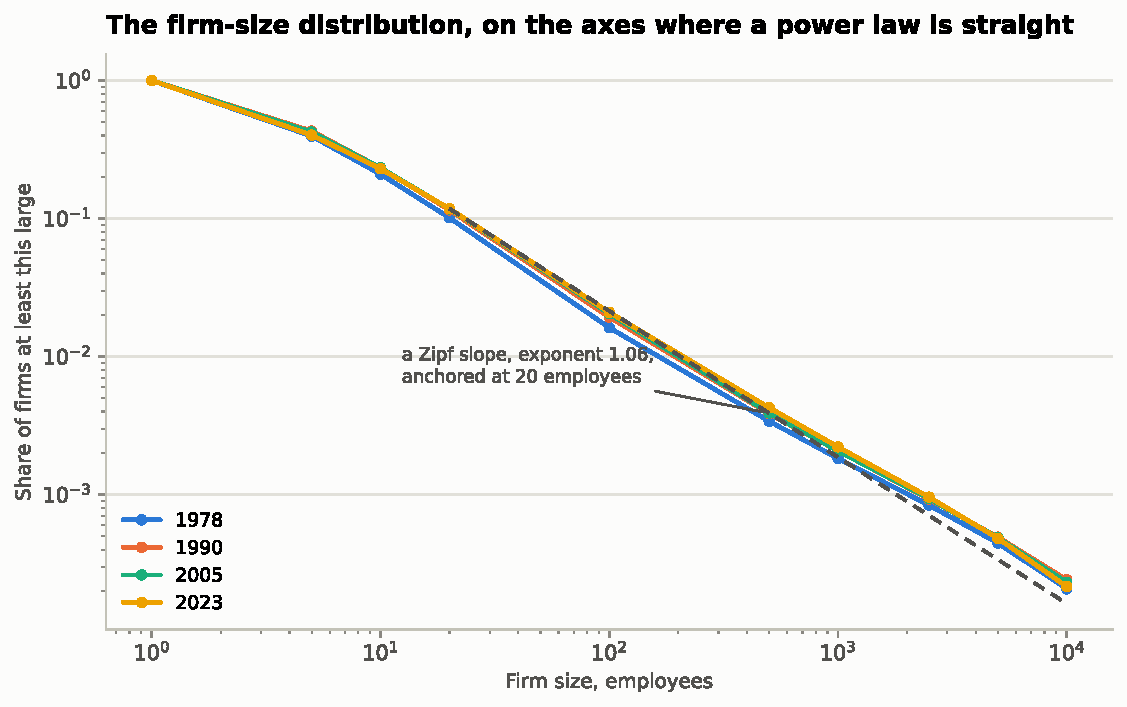
\includegraphics[width=0.85\textwidth]{figures/fig_survival.pdf}
\caption{The firm-size distribution on log-log axes, where a power law is a straight line.
Points are plotted at the lower edge of each of the ten published size classes. The dashed
reference has the Zipf slope of 1.06 and is anchored to the data at twenty employees, so the
comparison is of slopes rather than of levels. Source: authors' calculations from BDS.}
\label{fig:survival}
\end{figure}

Table~\ref{tab:model_comparison} reports the fits. The log-normal is preferred by Vuong's
test in all forty-six years of the sample, with $|Z|$ between 202 and 273 and never
approaching the region in which the data would be unable to separate the models. The Akaike
difference agrees at every date. The Pareto exponent fitted across the whole range is between 0.65 and 0.69 throughout,
below the unity at which the mean becomes infinite. That value should be read as the fit
failing rather than as an estimate of anything.

\begin{table}[H]
\caption{Pareto and log-normal fitted to the same ten bins by interval-censored maximum
likelihood, selected years. $\Delta$AIC is Pareto minus log-normal, so a positive value
favours the log-normal. The Vuong statistic tests the two non-nested models directly; a
value below $-1.96$ favours the log-normal and above $+1.96$ the Pareto, and values
between the two mean the data cannot separate them. The log-normal is preferred in all
46 years of the sample, in every case decisively. Source: authors' calculations from BDS.}
\label{tab:model_comparison}
\begin{tabular}{lrrrrrr}
\toprule
Year & Firms & $\hat\alpha$ & $\hat\mu$ & $\hat\sigma$ & $\Delta$AIC & Vuong $Z$ \\
\midrule
1978 & 3,577,193 & 0.6927 & -0.310 & 2.002 & 1.99e+05 & $-$202.5 \\
1985 & 4,081,789 & 0.6749 & -0.071 & 1.950 & 2.63e+05 & $-$232.1 \\
1990 & 4,459,635 & 0.6534 & 0.117 & 1.925 & 3.27e+05 & $-$262.5 \\
1995 & 4,688,220 & 0.6614 & -0.076 & 1.988 & 3.06e+05 & $-$252.7 \\
2000 & 4,913,068 & 0.6487 & -0.021 & 1.999 & 3.35e+05 & $-$268.2 \\
2005 & 5,176,905 & 0.6558 & -0.106 & 2.016 & 3.35e+05 & $-$272.0 \\
2010 & 5,027,027 & 0.6637 & -0.232 & 2.047 & 3.02e+05 & $-$255.4 \\
2015 & 5,158,865 & 0.6602 & -0.410 & 2.128 & 2.85e+05 & $-$253.7 \\
2020 & 5,345,576 & 0.6579 & -0.530 & 2.181 & 2.81e+05 & $-$255.5 \\
2023 & 5,604,596 & 0.6681 & -0.693 & 2.214 & 2.7e+05 & $-$251.0 \\
\bottomrule
\end{tabular}
\end{table}


C1 fails, decisively and in every year. This is not a marginal or sample-dependent result:
it is obtained on counts running from 3.58 million firms in 1978 to 5.60 million in 2023, at
a test statistic two orders of magnitude beyond conventional significance.

The reason the failure is interesting rather than merely negative is where it occurs.
Figure~\ref{fig:modelfit} plots both fitted models against the observed class shares for the
final year, with the ratio of predicted to observed beneath. The log-normal tracks the
observed distribution closely through the first five classes and then falls away; the Pareto
does the opposite, tracking the upper classes while overshooting the body by an order of
magnitude. Table~\ref{tab:topbin} states the same failure as a count. In 2023 there were
1{,}210 US firms with 10{,}000 employees or more. The log-normal that wins the likelihood
comparison expects 57. A single Pareto fitted across the whole range expects 11{,}916.

\begin{figure}[H]
\centering
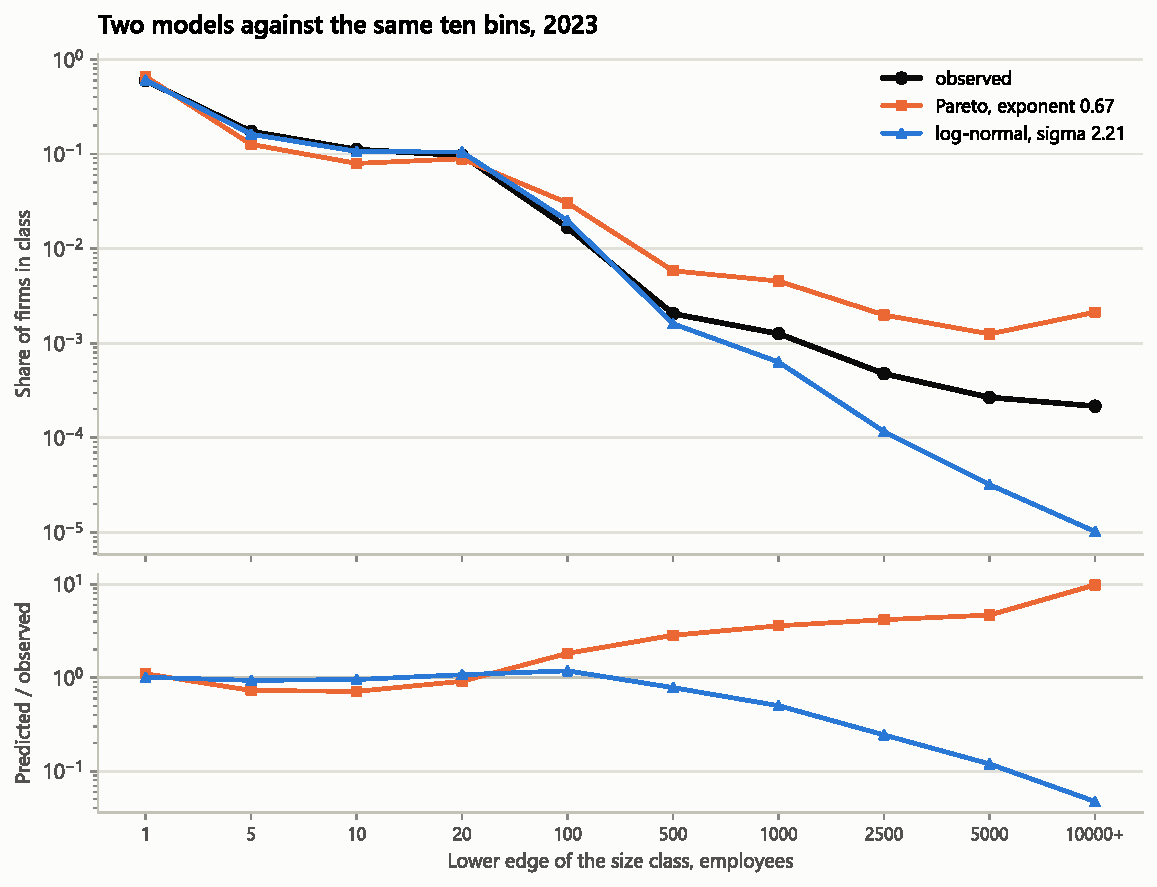
\includegraphics[width=0.86\textwidth]{figures/fig_model_fit.pdf}
\caption{(\textbf{a}) Observed share of firms in each size class, 2023, against the fitted
Pareto and the fitted log-normal, on a logarithmic vertical scale. (\textbf{b}) The ratio of
predicted to observed for each model. A value of one is exact agreement. The log-normal
holds through the body and collapses at the top; the Pareto does the reverse. Source:
authors' calculations from BDS.}
\label{fig:modelfit}
\end{figure}

\begin{table}[H]
\caption{Firms of 10{,}000 employees and over: the count each fitted model has to
explain. The log-normal wins the likelihood comparison of Table~\ref{tab:model_comparison}
in every year and under-predicts this class by a factor of 21 in the final year; a single
Pareto fitted across the whole range over-predicts it by an order of magnitude. Neither
model is the distribution, and the failure is on opposite sides. Source: authors'
calculations from BDS.}
\label{tab:topbin}
\begin{tabular}{lrrrrr}
\toprule
 & & \multicolumn{2}{c}{Predicted} & \multicolumn{2}{c}{Observed / predicted} \\
\cmidrule(lr){3-4}\cmidrule(lr){5-6}
Year & Observed & Log-normal & Pareto & Log-normal & Pareto \\
\midrule
1978 & 744 & 8 & 6,064 & 91.5 & 0.12 \\
1990 & 1,078 & 10 & 10,856 & 109.1 & 0.10 \\
2000 & 1,296 & 19 & 12,484 & 67.1 & 0.10 \\
2010 & 1,182 & 22 & 11,127 & 54.0 & 0.11 \\
2023 & 1,210 & 57 & 11,916 & 21.1 & 0.10 \\
\bottomrule
\end{tabular}
\end{table}


Neither model is the distribution. The log-normal wins on likelihood because most firms are
small and it describes the small firms well; it is wrong by a factor of twenty-one about the
firms that hold the economy's employment. Reporting only the model comparison would
therefore be misleading, which is why Table~\ref{tab:topbin} accompanies it.

\subsection{The Tail Is a Power Law, and Its Exponent Is Axtell's}
\label{subsec:tailresults}

Refitting the Pareto from progressively higher thresholds separates the two regimes.
Table~\ref{tab:thresholds} and the left panel of Figure~\ref{fig:tail} report the sweep.
Fitted from the smallest firm the exponent is 0.67; from ten employees upward it is 1.00;
from twenty employees upward it is 1.056; and it remains within roughly five hundredths of
unity at every higher threshold. The data does not support a single exponent. What it supports is a function of where the
fitting region starts, and that function settles near one exactly where the log-normal
begins to fail.

\begin{table}[H]
\caption{Pareto exponent refitted from progressively higher thresholds, the
\citet{ClausetShaliziNewman2009} procedure adapted to interval-censored data. The column
head is the lower bound of the fitting region in employees. Fitted from the smallest firm
the exponent is far below unity, which is the signature of a body the model does not
describe; from ten employees upward it sits near one at every threshold. Axtell's
(\citeyear{Axtell2001}) microdata estimate of 1.06 is reproduced at a threshold of twenty
employees. Source: authors' calculations from BDS.}
\label{tab:thresholds}
\begin{tabular}{lrrrrrrrr}
\toprule
Year & $\geq$1 & $\geq$5 & $\geq$10 & $\geq$20 & $\geq$100 & $\geq$500 & $\geq$1000 & $\geq$2500 \\
\midrule
1978 & 0.693 & 0.988 & 1.072 & 1.102 & 0.952 & 0.897 & 0.895 & 0.975 \\
1990 & 0.653 & 0.961 & 1.043 & 1.084 & 0.977 & 0.900 & 0.905 & 0.953 \\
2000 & 0.649 & 0.937 & 1.020 & 1.066 & 0.971 & 0.878 & 0.878 & 0.971 \\
2010 & 0.664 & 0.945 & 1.027 & 1.054 & 0.981 & 0.911 & 0.915 & 0.989 \\
2023 & 0.668 & 0.906 & 1.002 & 1.056 & 0.979 & 0.952 & 0.960 & 1.045 \\
\bottomrule
\end{tabular}
\end{table}


That value is the result we regard as the paper's strongest single number.
\citet{Axtell2001} obtained an exponent indistinguishable from unity, 1.059, from the US
firm census at the level of individual firms. We obtain 1.056 from ten published bins, on a
sample spanning forty-six years rather than one, using an estimator that never sees a firm.
Two very different instruments, one microdata and one interval-censored aggregate, agree to
three thousandths.

\begin{figure}[H]
\centering
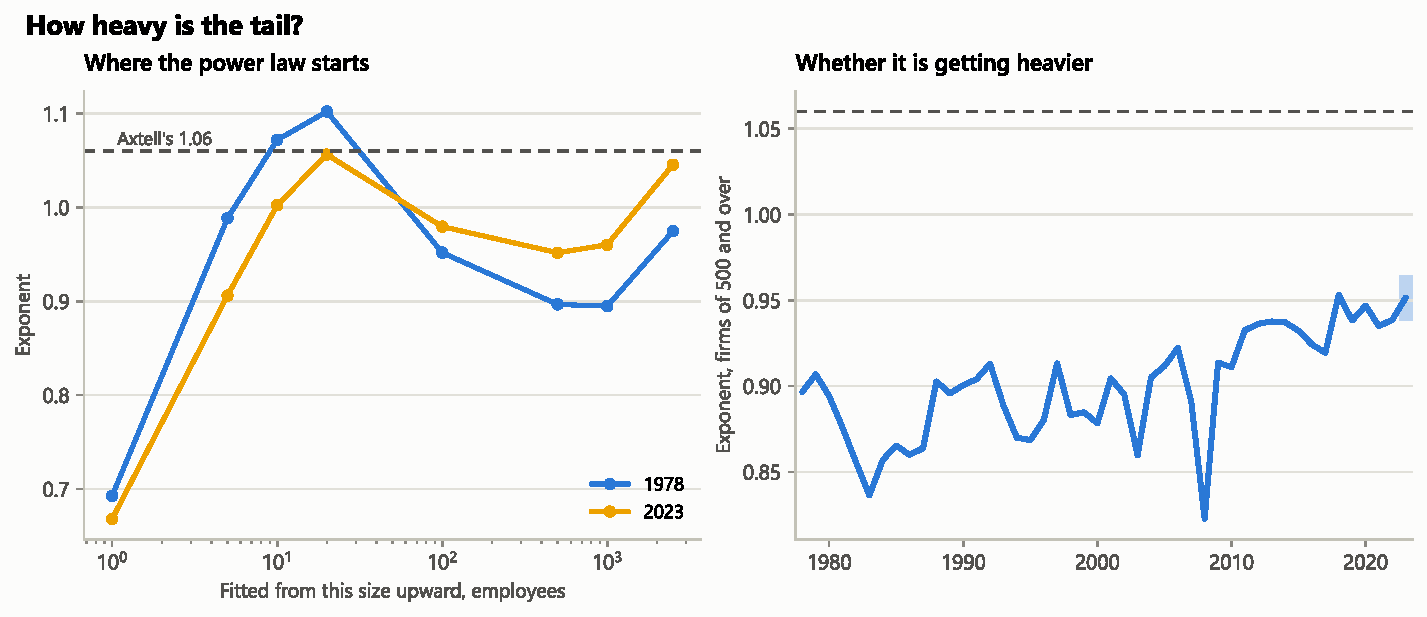
\includegraphics[width=\textwidth]{figures/fig_tail_exponent.pdf}
\caption{(\textbf{a}) The Pareto exponent as a function of the size threshold from which it
is fitted, for the first and last years of the sample. The dashed line is
\citeauthor{Axtell2001}'s (\citeyear{Axtell2001}) microdata estimate of 1.06. (\textbf{b})
The exponent fitted from 500 employees upward, by year, with the 95 per cent bootstrap
interval for the final year shaded. Source: authors' calculations from BDS.}
\label{fig:tail}
\end{figure}

C2 holds. The right panel of Figure~\ref{fig:tail} adds the time dimension, and it carries a
result that cuts against the direction the argument is usually made in: the tail became
\emph{lighter} over the period, the exponent above 500 employees rising from 0.897 in 1978
to 0.952 in 2023. There are not proportionally more very large firms than there were.
Section~\ref{subsec:tension} takes up what that means alongside the concentration results,
which move the other way.

Table~\ref{tab:robustness} states what the exponent is and is not sensitive to. The bootstrap
interval for the final year is 0.026 wide. Moving the open class's boundary by a factor of
two moves the estimate by 0.047, nearly twice as far, and varying the fitting threshold above
ten employees moves it by 0.077. Specification dominates sampling here. We therefore quote
the exponent to two decimals, treat differences smaller than about a tenth as
uninterpretable, and rest the distributional conclusion on the model comparison of
Section~\ref{subsec:c1}, which is not subject to any of this.

\begin{table}[H]
\caption{What the tail exponent is sensitive to. The bootstrap interval is the 95 per cent
percentile interval from 400 multinomial resamples of the final year's bin counts and
measures sampling noise alone. The threshold and boundary rows measure specification. The
exponent is more sensitive to where the fitting region starts, and to where the open class
begins, than it is to sampling, which is why the paper reports it to two decimals and rests
its distributional claim on the model comparison rather than on the exponent's level.
Source: authors' calculations from BDS.}
\label{tab:robustness}
\begin{tabular}{llr}
\toprule
Source of variation & Range examined & Spread in $\hat\alpha$ \\
\midrule
Sampling & 400 bootstrap resamples, 2023 & 0.0261 \\
Open-class boundary & 10{,}000 against 20{,}000 employees & 0.0474 \\
Fitting threshold & 10 to 2{,}500 employees & 0.1045 \\
Fitting threshold, including the body & 1 to 2{,}500 employees & 0.3880 \\
\bottomrule
\end{tabular}
\end{table}


\subsection{Dynamism Fell While Concentration Rose}
\label{subsec:dynamism}

Table~\ref{tab:dynamism} reports the movements in the firm population that the distributional
results sit inside. Establishment entry fell from 15.15 per cent to 10.61 per cent between
1978 and 2023, a decline of 4.54 points. Exit fell too, but by only 1.74 points, and from a
peak in 1982 rather than at the start. The turnover of American business slowed
asymmetrically: fewer firms are being born, not more are dying.

\begin{table}[H]
\caption{Dynamism and concentration in the universe of US employer firms. Entry and exit
are establishment rates. The size shares are of national employment and are computed on the
ten-class partition of Table~\ref{tab:bins}; the two largest classes are firms of 5{,}000
employees and over and the three smallest are firms under twenty. Age shares begin in 1982
because the Business Dynamics Statistics begins in 1978 and a firm cannot be observed at
age four before then. Source: authors' calculations from BDS.}
\label{tab:dynamism}
\begin{tabular}{lrrrr}
\toprule
 & First & Last & Change & Peak \\
\midrule
\multicolumn{5}{l}{\emph{Establishment turnover, per cent, 1978--2023}} \\
Entry rate & 15.15 & 10.61 & $-$4.54 & 15.15 (1978) \\
Exit rate & 11.14 & 9.40 & $-$1.74 & 12.38 (1982) \\
\addlinespace
\multicolumn{5}{l}{\emph{Share of national employment, per cent, 1978--2023}} \\
Two largest size classes & 30.16 & 35.69 & $\phantom{-}$5.53 & 35.76 (2021) \\
Three smallest size classes & 22.72 & 16.69 & $-$6.03 & 22.72 (1978) \\
\addlinespace
\multicolumn{5}{l}{\emph{Held by firms under five years old, per cent, 1982--2023}} \\
Share of firms & 39.21 & 31.93 & $-$7.28 & 40.96 (1987) \\
Share of employment & 13.50 & 8.94 & $-$4.56 & 15.92 (1988) \\
Share of job creation & 35.28 & 24.40 & $-$10.88 & 37.28 (1987) \\
\bottomrule
\end{tabular}
\end{table}


Over the same period the share of national employment held by the two largest size classes
rose from 30.16 per cent to 35.69 per cent, and the share held by the three smallest fell
from 22.72 to 16.69. The two movements are close to mirror images. The class-level Herfindahl
rose from 0.1406 to 0.1572, which by the argument of Section~\ref{subsec:concentration} is a
floor on the firm-level index and is interpreted only in direction.

The age series, which begins in 1982, is the sharpest of the three. Firms under five years
old held 39.21 per cent of all firms in 1982 and 31.93 per cent in 2023; 13.50 per cent of
employment and 8.94 per cent; and 35.28 per cent of gross job creation against 24.40 per
cent. All three peak in the late 1980s. The largest proportional decline is in job creation,
which is the channel through which young firms matter most.

Figure~\ref{fig:dynamism} places entry and the large-firm employment share on a common time
axis in separate panels. The two series correlate at $-0.770$ over forty-six years. Both
trend, and we report the figure as description; nothing causal follows from it, and
Section~\ref{subsec:guards} states why.

\begin{figure}[H]
\centering
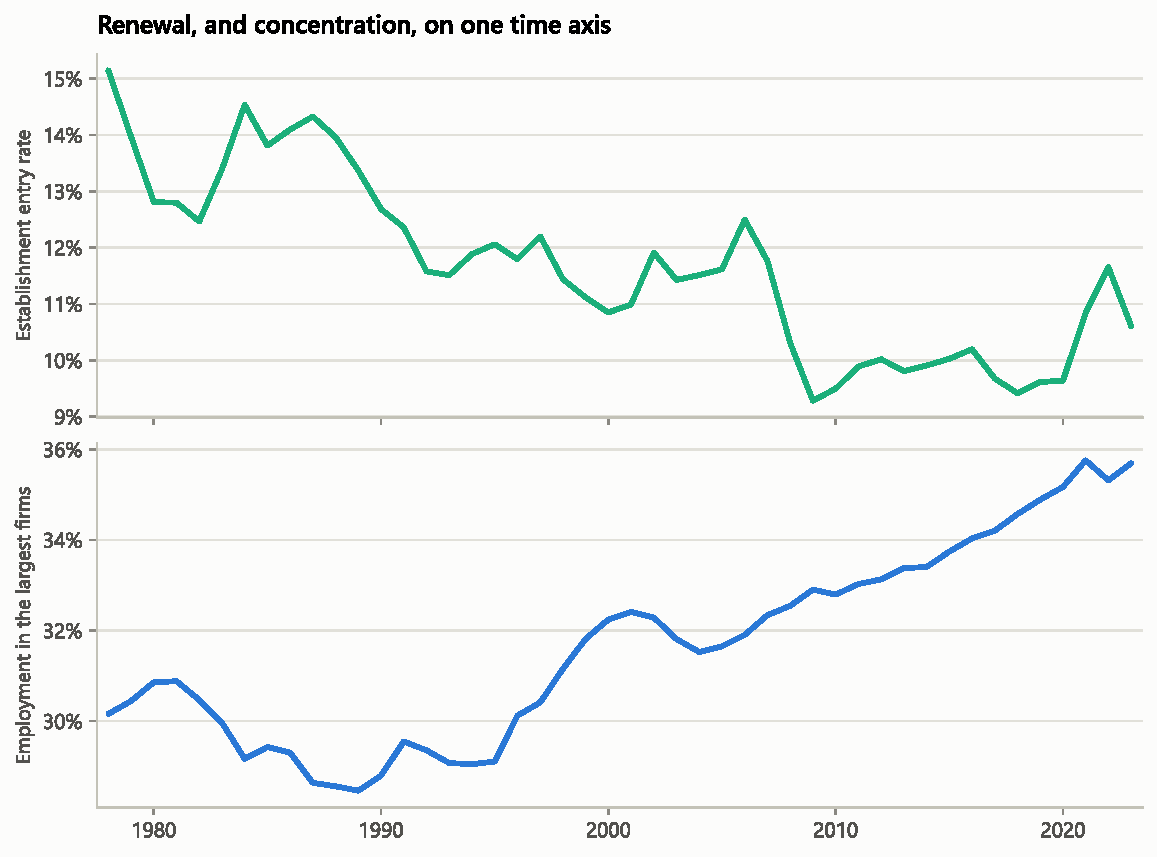
\includegraphics[width=0.80\textwidth]{figures/fig_dynamism.pdf}
\caption{(\textbf{a}) Establishment entry rate. (\textbf{b}) Share of national employment
held by the two largest firm-size classes. The two panels share a time axis and are drawn
on separate vertical scales deliberately: the quantities have different units and plotting
them against a common axis would make the comparison a matter of the author's choice of
scaling. Source: authors' calculations from BDS.}
\label{fig:dynamism}
\end{figure}

\subsection{Concentration Rose Inside Sectors, Not Between Them}
\label{subsec:c3a}

Table~\ref{tab:shiftshare} and Figure~\ref{fig:shiftshare} report the decomposition of
Equation~\eqref{eq:shiftshare} across nineteen NAICS sectors over 1978 to 2023.

\begin{table}[H]
\caption{Shift-share decomposition of the change in the share of employment held by the two
largest firm-size classes, 1978 to 2023, across 19 NAICS sectors. The three terms sum to the
observed change by construction and the identity was asserted in code. The within term is
what the change would have been had sector employment weights not moved; the between term
is what it would have been had concentration inside each sector not moved. Source: authors'
calculations from BDS.}
\label{tab:shiftshare}
\begin{tabular}{lr}
\toprule
Component & Percentage points \\
\midrule
Within sectors & $\phantom{-}$6.25 \\
Between sectors & $-$6.38 \\
Interaction & $\phantom{-}$5.66 \\
\midrule
Total, equal to the observed change & $\phantom{-}$5.53 \\
\bottomrule
\end{tabular}
\end{table}


The observed change of $+5.53$ percentage points decomposes into $+6.25$ points occurring
inside sectors, $-6.38$ points from employment moving between them, and $+5.66$ points of
interaction. The between term is large and negative. Employment moved \emph{toward} less concentrated
sectors, among them retail, health care and administrative services, over the same decades in
which the economy-wide large-firm share rose. Sectoral composition
worked against the trend and lost.

\begin{figure}[H]
\centering
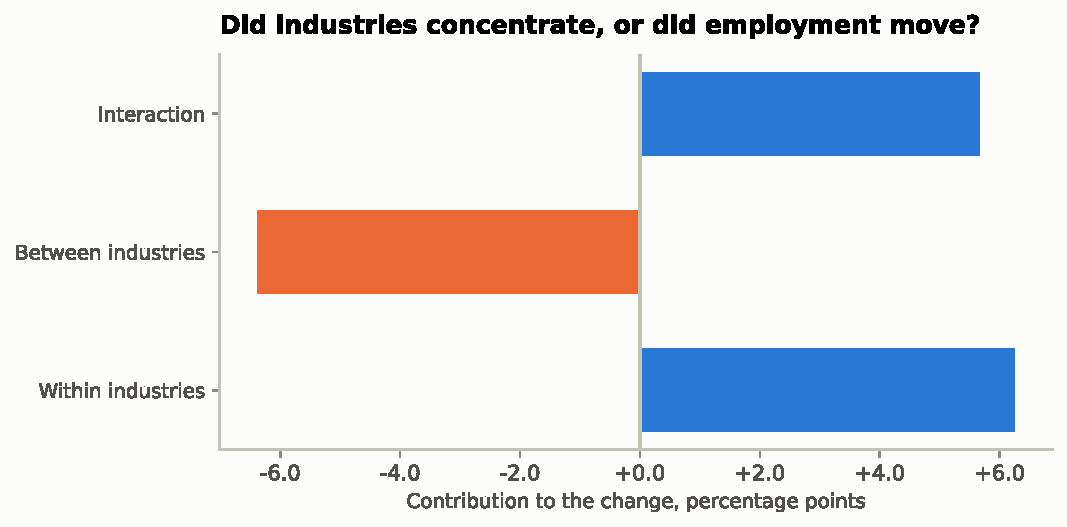
\includegraphics[width=0.78\textwidth]{figures/fig_shiftshare.pdf}
\caption{Shift-share decomposition of the change in the share of employment held by the two
largest firm-size classes, 1978 to 2023, across nineteen NAICS sectors. The three
contributions sum to the observed change of $+5.53$ percentage points by construction.
Source: authors' calculations from BDS.}
\label{fig:shiftshare}
\end{figure}

This is the first half of the case against C3, and it is a decomposition rather than a
correlation, so it does not depend on a specification. The interaction term is nearly as
large as the within term, which is what forty-six years does to a decomposition of this kind,
and the three terms are accordingly not read as separable causes. What can be read from them
is the sign of the between term, and that sign is unambiguous.

\subsection{Size Buys No Margin}
\label{subsec:creation}

The second half of the case against C3 concerns profit rather than employment.
Figure~\ref{fig:creation} plots, for each of the 71 industries and for the most recent year
in which the components of value added are published, how much value the industry adds
against the share of that value it keeps as operating surplus.

\begin{figure}[H]
\centering
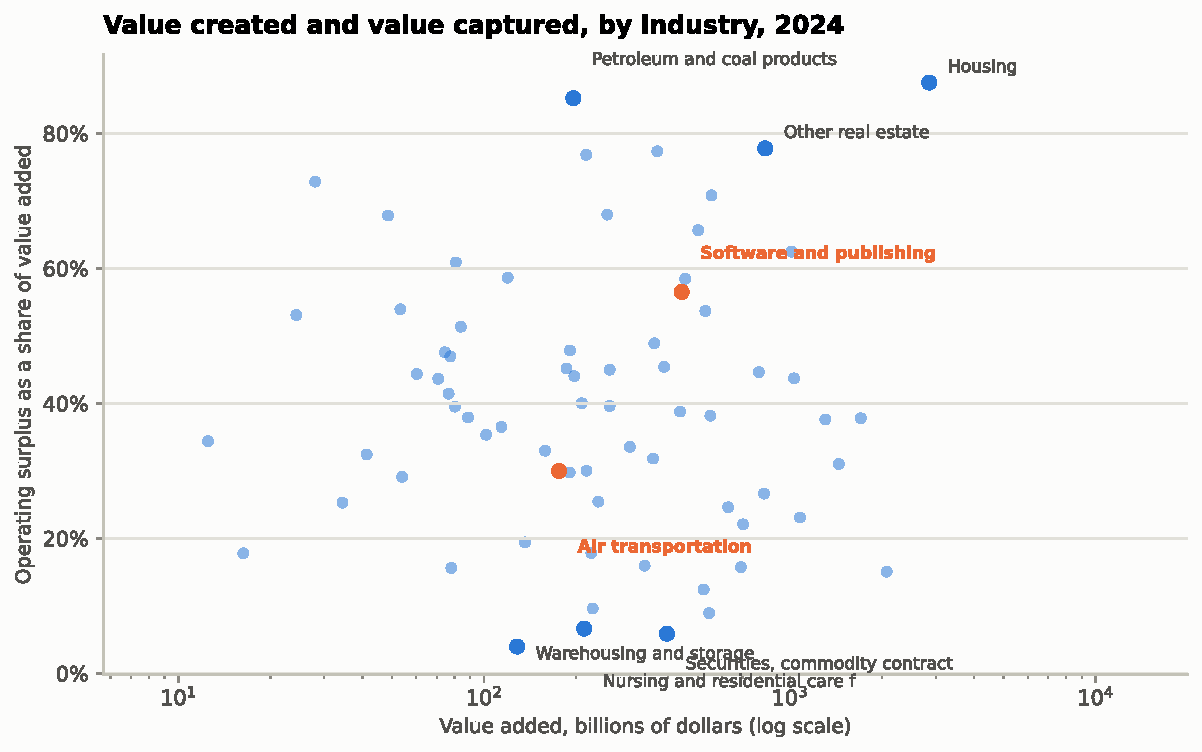
\includegraphics[width=\textwidth]{figures/fig_creation_capture.pdf}
\caption{Value created against value captured across 71 industries, 2024. The horizontal
axis is value added on a logarithmic scale; the vertical axis is gross operating surplus as
a share of value added. Air transportation and the software and publishing industries are
marked. Source: authors' calculations from the GDP-by-Industry accounts.}
\label{fig:creation}
\end{figure}

There is no relationship. The correlation between log value added and the capture rate is
0.009 by Pearson and $-0.047$ by Spearman across 71 industries. Capture varies enormously, from under 4 per cent to over 87 per cent as
Table~\ref{tab:capture} shows, but it does not vary with size. An industry's scale carries no information about the share of its own output it
retains.

\begin{table}[H]
\caption{Capture rates at the extremes, 2024, and the association between creating value and
keeping it. Capture is gross operating surplus as a share of value added. The correlation
is computed against log value added across all 71 industries. Both extremes are partly
artefacts of the tax and subsidy treatment rather than of profitability, which is why the
paper rests on the association and not on the ranking. Source: authors' calculations from
the GDP-by-Industry accounts.}
\label{tab:capture}
\begin{tabular}{lr}
\toprule
Industry & Capture, per cent \\
\midrule
\multicolumn{2}{l}{\emph{Highest}} \\
Housing & 87.5 \\
Petroleum and coal products & 85.2 \\
Other real estate & 77.8 \\
Rental and leasing services and lessors of intangible assets & 77.3 \\
Farms & 76.8 \\
\addlinespace
\multicolumn{2}{l}{\emph{Lowest}} \\
Warehousing and storage & 4.0 \\
Securities, commodity contracts, and investments & 5.9 \\
Nursing and residential care facilities & 6.6 \\
Management of companies and enterprises & 8.9 \\
Social assistance & 9.6 \\
\midrule
\multicolumn{2}{l}{\emph{Association of size with capture, 71 industries}} \\
Pearson correlation, log value added with capture & $\phantom{-}$0.009 \\
Spearman rank correlation & $-$0.047 \\
\bottomrule
\end{tabular}
\end{table}


Both extremes of that ranking are partly artefacts. Surplus plus compensation reaches 134
per cent of value added for government enterprises and 129 per cent for farms, because net
taxes on production are negative where subsidies are large, and it falls to 20 per cent for
funds and trusts at the other end. The ranking is therefore reported for transparency and
the finding rests on the association, which does not depend on the tails: dropping the five
highest and five lowest industries leaves the correlation statistically indistinguishable
from zero.

\subsection{Capture Concentrates Faster Than Creation}
\label{subsec:captureresults}

The one dimension on which the sectoral picture does concentrate is the distribution of
surplus itself, and it does so faster than the distribution of value added.
Table~\ref{tab:concentration} and Figure~\ref{fig:top10} report both.

\begin{table}[H]
\caption{Concentration of value created and value captured across 71 industries that tile
the economy exactly once, 1997 to 2024. Value added measures creation and gross operating
surplus measures capture. Capture is more concentrated than creation in every year of the
sample and its concentration rises further over the period. Both series peak in 2020.
Source: authors' calculations from the GDP-by-Industry accounts.}
\label{tab:concentration}
\begin{tabular}{lrrr}
\toprule
Measure & 1997 & 2024 & Change \\
\midrule
Gini, value added & 0.512 & 0.551 & $\phantom{-}$0.039 \\
Gini, operating surplus & 0.587 & 0.627 & $\phantom{-}$0.040 \\
\addlinespace
Top ten industries, value added, per cent & 45.21 & 48.34 & $\phantom{-}$3.13 \\
Top ten industries, operating surplus, per cent & 50.96 & 55.60 & $\phantom{-}$4.64 \\
\bottomrule
\end{tabular}
\end{table}


Between 1997 and 2024 the Gini of value added across industries rose from 0.512 to 0.551 and
the Gini of operating surplus from 0.587 to 0.627. The top ten industries' share of value
added rose 3.13 points against 4.64 points for surplus. Capture is more concentrated than
creation in every year of the sample, and the gap widens.

\begin{figure}[H]
\centering
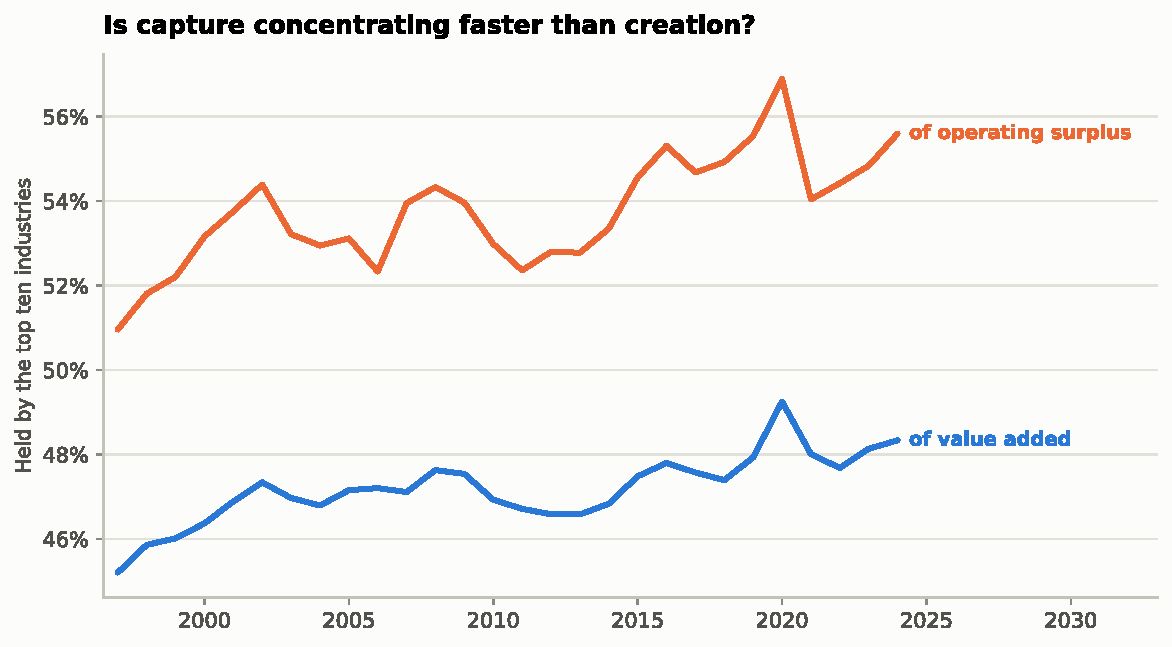
\includegraphics[width=0.82\textwidth]{figures/fig_top10.pdf}
\caption{Share of value added and of gross operating surplus held by the ten largest of 71
industries, 1997 onward. Value added runs to 2025 and surplus to 2024, the last year for
which the components of value added are published. Source: authors' calculations from the
GDP-by-Industry accounts.}
\label{fig:top10}
\end{figure}

Two qualifications attach to this result and neither is small. Both series peak in 2020, so
the size of the change depends on the endpoint chosen; the ordering, that surplus is more
concentrated than value added, holds in every year and does not. And these are industries,
not firms, so by the argument of Section~\ref{subsec:unit} the figures are floors on the
concentration of profit among companies and are not estimates of it.

%%%%%%%%%%%%%%%%%%%%%%%%%%%%%%%%%%%%%%%%%%
\section{Discussion}
\label{sec:discussion}

\subsection{What the Three Results Establish Together}
\label{subsec:together}

Taken separately, each result is a modest empirical finding. Taken together they identify
the level at which the phenomenon lives, which is the paper's contribution.

The power law is real, and it is a property of the tail. The exponent above twenty employees
is 1.056, agreeing with a microdata estimate obtained by a completely different method. But
the distribution as a whole is not a power law, and it is not close: the log-normal wins in
all forty-six years at $|Z|$ above 200. Most American firms are not in the tail and are not
governed by it. The two facts are compatible because the distribution is a mixture, and
statements that treat "the firm size distribution is a power law" as a single claim are
conflating them.

The power law is also not a property of sectors. If it were, an industry's identity would
predict what its firms keep, and it does not: the association between creating value and
keeping it is 0.009. And if rising concentration were compositional, with the economy
tilting toward industries that were always concentrated, the between-sector term of the
decomposition would carry it. Instead that term is $-6.38$ points against $+6.25$ inside
sectors. Concentration rose inside industries while employment moved toward less
concentrated ones.

The unit at which the phenomenon operates is therefore the firm, within its industry, in the
upper tail. That is a narrower object than the sectoral aggregates on which most public
argument about the digital economy is conducted, and it is systematically invisible to them.

\subsection{Why Sector Averages Mislead, Specifically}
\label{subsec:unit}

The mechanism is worth stating precisely, because ``aggregation bias'' is too general a
phrase to be useful and the failures here are nameable.

The first is arithmetic. An industry average is a weighted mean over its firms, and a mean
is exactly the statistic that a heavy tail is least well described by. An industry
containing one firm that captures most of the surplus and twenty that capture almost none
reports the same number as an industry in which twenty-one firms each capture a middling
share. Section~\ref{subsec:c1} showed that the firm distribution is heavy-tailed at the top;
it follows immediately that industry means discard the part of the distribution that
generates the phenomenon.

The second is that the measures available at industry level are contaminated in ways that do
not average out. Value added over gross output, an obvious candidate for a margin, tracks
vertical integration: air transportation scores above most software industries on it.
Operating surplus contains depreciation, net interest and proprietors' income. Net taxes on
production go negative where subsidies are large, which puts farms and government
enterprises above 100 per cent of value added on the capture measure. Each of these is a
specific, identifiable reason a sector comparison misleads, and none is fixed by using a
different sector classification.

The third is the censoring of Table~\ref{tab:censoring}. Every public instrument stops
resolving below the point at which the tail becomes interesting. Because grouping can only
reduce a concentration index, every figure reported here is a floor. The direction of the
bias is known; its magnitude is not, and cannot be established from these sources.

\subsection{The Tension Between a Lighter Tail and Rising Concentration}
\label{subsec:tension}

Two of our results appear to point in opposite directions, and we take the apparent conflict
seriously rather than reporting only the convenient half.

The tail exponent above 500 employees rose from 0.897 to 0.952 over 1978 to 2023, meaning the
tail became lighter: relative to the whole population there are not more very large firms
than there used to be. Over the same years the share of employment in the largest classes
rose 5.53 points and the class-level Herfindahl rose, meaning employment concentrated.

These measure different objects and are not in contradiction. The first is a statement about
the count of firms at each size; the second is about the share of workers those firms employ.
A distribution can flatten slightly in its count of large firms while the largest of them
grow relative to the economy. What the pair rules out is the simplest story, in which
concentration rose because the number of giant firms multiplied. It did not. The existing
large firms took a larger share.

Read alongside Table~\ref{tab:dynamism}, that suggests the composition of the tail matters
more than its thickness. Entry fell by 4.54 points and the share of job creation held by
firms under five years old fell by 10.88; entry is the mechanism by which a new firm reaches
the tail, and it has weakened substantially. We state this as an interpretation the results
are consistent with, not as a finding: nothing in our data tracks individual firms into or
out of the tail, and establishing it would require the longitudinal microdata we do not
have.

\subsection{What Would Have Falsified the Argument}
\label{subsec:falsify}

Three specific outcomes would have overturned the paper's claim, and it is worth recording
that each was tested rather than avoided.

Had the Vuong statistic fallen inside $\pm 1.96$, the data would have been unable to
distinguish the two distributions and no claim about the shape could have been made. It did
not, in any year.

Had the between-sector term of the shift-share been the large positive one, rising
concentration would have been a compositional fact about which industries grew, and the
sectoral reading would have been correct. The term is negative and roughly equal in magnitude
to the within term.

Had capture correlated with industry size, the sectoral reading would again have been
supported: large industries would systematically keep more. The correlation is 0.009.

We note in the same spirit that the paper's negative results are reported at the same weight
as its positive ones. The value-added margin does not measure what we hoped it would and is
withdrawn. The whole-distribution Pareto exponent of roughly 0.67 is reported as evidence of
a failed fit rather than quietly dropped. And the tail exponent's sensitivity to
specification, which exceeds its sampling uncertainty by roughly a factor of two, is stated
in Table~\ref{tab:robustness} rather than left for a reader to discover.

\subsection{Limitations}
\label{subsec:limits}

The central limitation is the one the paper is partly about. We never observe a firm. Every
result rests on grouped or aggregated data, and while the grouping is handled with an
estimator appropriate to it, no amount of estimation recovers what the tabulation did not
record. Between-industry concentration is a floor on between-firm concentration and never an
estimate of it.

Four narrower limitations qualify specific results. The tail exponent is more sensitive to
the position of the open class boundary than to sampling, so differences below about a tenth
are not interpretable. The firm-age series begins in 1982 and cannot be extended back. The
concentration comparison of Section~\ref{subsec:captureresults} peaks in 2020, so its
magnitude is endpoint-dependent even though its ordering is not. And the shift-share is
computed over a forty-six-year window, which produces an interaction term nearly as large as
the within term and precludes reading the three components as separable causes.

Finally, the association reported in Section~\ref{subsec:creation} is a single cross-section
on one definition of capture at one level of aggregation. It is what the accounts show, and
it is consistent across the years we examined, but it is not a general law about size and
profitability and is not offered as one.

%%%%%%%%%%%%%%%%%%%%%%%%%%%%%%%%%%%%%%%%%%
\section{Future Scope}
\label{sec:future}

The obvious next step is the one the data prevented. Every claim in this paper about firms
within industries is inferred from bounds; the Census Bureau's Longitudinal Business Database
and the restricted-access microdata behind the GDP-by-Industry accounts contain the firm-level
observations that would turn those bounds into estimates. The specific question is whether
the within-industry dispersion of capture is heavy-tailed in the way the size distribution's
upper tail is, and how much of the between-industry concentration reported in
Section~\ref{subsec:captureresults} is a within-industry phenomenon showing through.
The apparatus in this paper is designed to transfer directly: the same likelihood, without
the interval censoring, and the same decomposition at a finer unit.

A second direction concerns the mechanism, which the estimates here do not deliver. Network
effects, scalable intangible capital, regulatory barriers to entry, and the acquisition of
young competitors before they mature all imply the pattern we observe, a heavy upper tail
whose composition renews more slowly than it once did. The published aggregates cannot tell
them apart. Linking the entry decline of Table~\ref{tab:dynamism} to the acquisition
record at industry level would begin to separate the last of these from the others.

A third is comparative. The partition-recovery procedure of Sections~\ref{subsec:partition}
and \ref{subsec:industries} needs nothing specific to the United States: it requires only a
grouped tabulation that publishes its own total. Eurostat's structural business statistics
and the OECD's business dynamics collections are tabulated the same way and would support the
same tests, which would establish whether the log-normal body with a Pareto tail, and the
absence of any relation between sectoral scale and sectoral capture, are features of the
American economy or of market economies generally.

A fourth follows from the tension in Section~\ref{subsec:tension}. Distinguishing a tail whose
membership churns from one whose membership is fixed requires following firms, not counting
them. Transition matrices between size classes are published for some of these collections
and would answer directly whether the slowing of entry has translated into a more static
upper tail.

Finally, the censoring documented in Table~\ref{tab:censoring} is itself a finding with a
constituency. The statistical agencies choose top-codes and terminal classes for disclosure
reasons that are sound, but the choices were made when the upper tail was thinner than it is
now, and they interact badly with the questions the digital-economy literature currently
asks. A systematic account of how much of the concentration literature's estimated magnitude
is attributable to these ceilings would be worth having, and this paper's bounds are a
starting point for it.

%%%%%%%%%%%%%%%%%%%%%%%%%%%%%%%%%%%%%%%%%%
\section{Conclusion}
\label{sec:conclusion}

The power law in American business is real, and it is narrower than it is usually made to
sound.

It is real in the upper tail of the firm size distribution, where the exponent above twenty
employees is 1.056. That is within three thousandths of the value \citet{Axtell2001} obtained
from firm-level microdata, reproduced here from ten published bins across forty-six years by
an estimator that never observes a firm. It is not a description of the distribution as a whole:
a log-normal is preferred in every year of the sample at $|Z|$ above 200, and the same fitted
log-normal under-predicts firms of 10{,}000 employees and over by a factor of twenty-one.
Both models fail, on opposite sides, and the distribution is a mixture of the two regimes.

It is not a property of sectors at all. Across 71 industries that tile the economy exactly
once, how much value an industry creates carries no information about the share of it the
industry keeps: 0.009 by Pearson, $-0.047$ by Spearman. And the forty-six-year rise in large-firm employment share was not compositional:
$+6.25$ percentage points of it occurred inside sectors while $-6.38$ points came from
employment moving toward less concentrated ones. What did concentrate at the sectoral level is capture rather than
creation: the Gini of operating surplus exceeds that of value added in every year and rose
further over the period.

The phenomenon operates on the firm, inside its industry, in the tail, which is
precisely the unit at which public statistics stop resolving. The largest
firm-size class is open at 10{,}000 employees, the household income survey top-codes at
\$200{,}000, occupational wages stop at the ninetieth percentile, and industry accounts
average over the firms they contain. Because grouping can only reduce a concentration index,
every figure in this paper is a floor, and so is every comparable figure in the literature
that draws on these sources.

For this question a sectoral statistic is a view of the wrong object, one in which the
dispersion that constitutes the phenomenon has already been averaged away. Policy addressed to concentrated \emph{industries} and policy addressed
to concentrated positions \emph{within} industries are different instruments, and the
evidence assembled here points at the second.

%%%%%%%%%%
\vspace{6pt}

\authorcontributions{Conceptualisation, S.P. and E.P.; methodology, S.P.; software,
S.P. and C.J.; validation, S.P., C.J. and E.P.; formal analysis, S.P.; data curation, S.P.
and C.J.; writing---original draft preparation, S.P.; writing---review and editing, C.J.
and E.P.; visualisation, S.P.; supervision, E.P. All authors have read and agreed to the
published version of the manuscript.}

\funding{This research received no external funding.}

\dataavailability{All data are public. The Business Dynamics Statistics is available from
the US Census Bureau API at \url{https://api.census.gov/data/timeseries/bds}; the
GDP-by-Industry accounts are available from the Bureau of Economic Analysis API at
\url{https://apps.bea.gov/api/data} under the \texttt{GDPbyIndustry} dataset. Both require a
free API key. Because both providers revise their series, and because the industry and
size-class partitions used here are recovered at run time rather than hard-coded, we deposit
the retrieved tabulations as CSV alongside the analysis notebooks, the recovered partitions
and their reconciliation gaps, the planted-answer validation output, every result table
reported here, and an environment lockfile recording the library versions and retrieval
dates. \todo{repository URL and archival DOI}}

\conflictsofinterest{The authors declare no conflicts of interest.}

\begin{adjustwidth}{-\extralength}{0cm}
\reftitle{References}
\bibliography{references}
\end{adjustwidth}

\end{document}
